This chapter focuses on the compositing techniques which include \emph{transformation} and \emph{blending} to get the final stitched image. We use two or more input images for stitching and we do not change the co-ordinates of \emph{reference image} and all other images (i.e. \emph{floating images}) are transformed into the reference image co-ordinates using \emph{homography}. Section~\ref{sec:transformation} discusses about \emph{transformation} which overlaps the common part of images. The resulting \emph{composite image} might contain visible seams (due to exposure differences), blur (due to mis-registration) and ghosting (due to moving objects). The quality of the stitched image is defined by the similarity of the stitched image to the input images and the visibility of seam between the images~\cite{levin:04}.

\section{Transformation}
\label{sec:transformation}
In this section, the transformation of images into the the co-ordinates of the reference image is carried out and we estimate the composite size and overlapped regions of the the images. The medical images are always flat without any radial distortion, homography can be used to transform the co-ordinates~\cite{Szeliski:06}.
\begin{description}
\item [\emph{Estimation of Composite Size}]
The estimation of the composite size is carried out by transforming the corners of the floating images. If we already know the direction of stitching (see section~\ref{sec:preprocessing}), then it is easy to estimate the size. We have to develop a general algorithm which works for any alignments. Since, most of the X-ray stitching problems, we already know the alignment (either vertical or horizontal) between images. So, we can modify the algorithm that uses direction information for faster estimation. A simple example on how to compute the composite size has been presented below:\\

\noindent Suppose, the transformed corners of the floating image are \{($x_{f1}$, $y_{f1}$), ($x_{f2}$, $y_{f2}$), ($x_{f3}$, $y_{f3}$), ($x_{f4}$, $y_{f4}$)\} and the corners of the reference image are \{($x_{r1}$, $y_{r1}$), ($x_{r2}$, $y_{r2}$), ($x_{r3}$, $y_{r3}$), ($x_{r4}$, $y_{r4}$)\}. Then, the corners of the composite image are calculated as follows:
\begin{enumerate}
	\item Calculate the minimum and maximum of x and y values of corners of transformed float image and reference image i.e.
	\begin{equation}
	\begin{split}
	x_{min}=min(x_{f1},x_{f2},x_{f3},x_{f4},x_{r1},x_{r2},x_{r3},x_{r4})\\
	y_{min}=min(y_{f1},y_{f2},y_{f3},y_{f4},y_{r1},y_{r2},y_{r3},y_{r4})\\
	x_{max}=max(x_{f1},x_{f2},x_{f3},x_{f4},x_{r1},x_{r2},x_{r3},x_{r4})\\
	y_{max}=max(y_{f1},y_{f2},y_{f3},y_{f4},y_{r1},y_{r2},y_{r3},y_{r4})	
	\end{split}
	\label{eq:minmax-composite-corners}
	\end{equation}

	\item Now the corners of the composite image are  {($x_{min}$, $y_{min}$), ($x_{max}$,$y_{min}$), ($x_{max}$, $y_{max}$), ($x_{min}$, $y_{max}$)}. Obviously, the width and height of the composite image will be ($x_{max}$-$x_{min}$) and ($y_{max}$-$y_{min}$) respectively. Unless the two images are exactly same, the composite image size is always greater the either image.

\begin{figure}[H]%
  \centering
	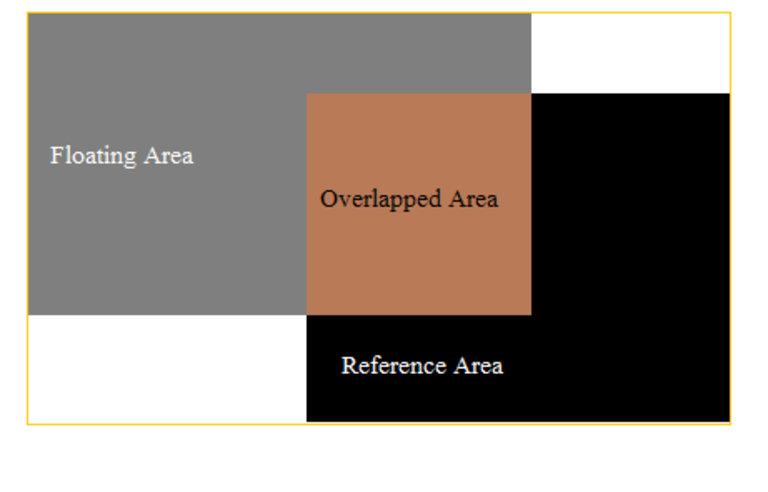
\includegraphics[width=\columnwidth]{2.mainmatter/2.Methodology/figures/Compositing}%
	\caption[Compositing]{Compositing of two images. The area within golden line is the compositing area. The gray area is floating image while black area is reference image.The overlapped area is painted with brown color.}%
	\label{fig:compositing-area}%
\end{figure}

\end{enumerate}

\item [\emph{Overlapping area identification}]
After we calculate the composite area i.e. the size of the stitched image, next task is to create an image with composite size and assign the pixel values of the float and reference images. Till now everything is okay except the overlapping areas. We assigned the overlapping pixels two times because those part is common to both floating and reference images (see figure~\ref{fig:compositing-area}). Since most of the real time problems, the overlapping areas are not same due to exposure differences and illumination which results visible seams in composite images. Again, we get blurred or ghosts in the overlapping region because of not accurate registration. To remedy these problem, we implement blending techniques. Some popular blending techniques are discussed in section~\ref{sec:blending}. Sometimes, if the intensity difference between images is large, the blending techniques are not capable of completely removing the visible seams~\cite{Dubrofsky:07}, we have to implement exposure compensation technique discussed in section~\ref{sec:exposure-compensation}.


\end{description}
\section{Blending}
\label{sec:blending}
The overlapping regions are blended for exposure compensation and mis-alignments. There are blending techniques which remove discontinuities in the composite image and create visually appealing stitched image. In this section, I am going to discuss some popular blending techniques: \emph{Optimal Seam Blending}, \emph{Alpha Blending} and \emph{Pyramid Blending}.
\subsection{Optimal Seam Blending}
\label{sec:optimal-seam-blending}
Optimal seam blending method search for a curve in the overlap region on which the difference of the images are minimal. If $I_1$ and $I_2$ are overlapping regions, for any y=$y_1$, a point (x,$y_1$) lies on the optimal seam curve if $I_1$(x,$y_1$) - $I_2$(x,$y_1$) is minimum for all x. Then, each image is copied to corresponding side of the seam. This simple method, however, does not give good result when there is global intensity difference between the images $I_1$ and $I_2$~\cite{levin:04}. 
\subsection{Alpha Blending}
\label{sec:alpha-blending}
Alpha blending, also called \emph{feathering}, is simple but effective algorithm. Alpha blending assigns the weight values (i.e. $\alpha$) to the pixels of the overlapping area. For $\alpha$=0.5, we get simple averaging, where both the overlapped areas will contribute equally to create stitched image. The value of $\alpha$ ranges from 0 to 1; if $\alpha$=0, then the pixel has no effect in composite region while $\alpha$=1 implies the pixel is copied there. Suppose, composite image $I$ is created from horizontally aligned images $I_1$ (left) and $I_2$ (right), then
\begin{equation}
I=\alpha I_1 + (1- \alpha)I_2
\label{eq:alpha-blending}
\end{equation}
Initially, we start with $\alpha$=1 (i.e. fully opaque) from $I_1$ until we reach overlap region. We go on decreasing $\alpha$ until it reaches to 0 (i.e. fully transparent) at the end of overlap region (see figure~\ref{fig:alpha-blending}).

\begin{figure}[H]%
\centering
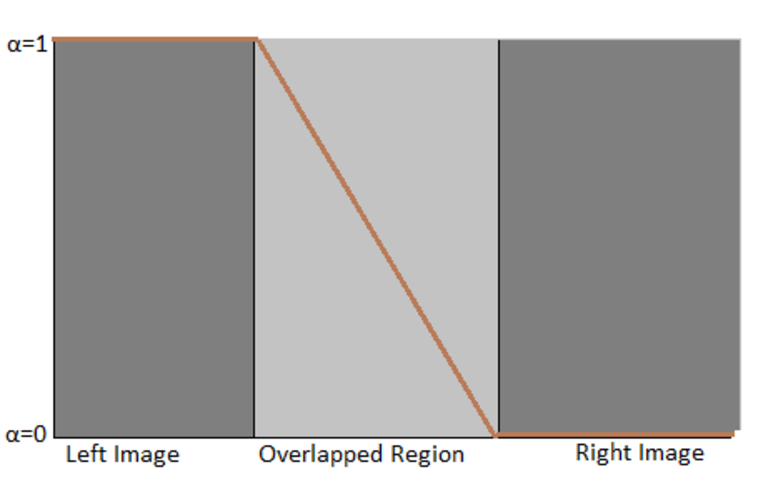
\includegraphics[width=0.9\columnwidth]{2.mainmatter/2.Methodology/figures/alpha-blending}%
\caption[Alpha Blending]{Alpha blending: $\alpha$ decreases from 1 to 0 in the overlapping region.}%
\label{fig:alpha-blending}%
\end{figure}

\noindent The above method is for horizontally aligned images; and similar technique can be used for vertically aligned images. If alignment is both horizontal and vertical, then left, right, top and bottom regions of the blending region will have effect in blending.\\

\noindent Alpha blending technique works well if the intensities of images $I_1$ and $I_2$ are similar. The advantage of alpha blending is its simplicity and we can tweak it to make it faster e.g. \emph{Look Up Table}~\cite{rankov:05}. 

%TODO The width of overlapped area effect in alpha blending
\subsection{Pyramid Blending}
\label{sec:laplacian-pyramid-blending}
The \emph{pyramid blending} uses image pyramids to blend and we use blending mask to mask the blended area. The blending mask assigns the weights of the pixels of the compositing images. The method consists of the following steps~\cite{Szeliski:06}:
\begin{itemize}
	\item Create Laplacian pyramids $L_1$ and $L_2$ from images $I_1$ and $I_2$.
	\item Create a Gaussian pyramid $G_M$ of the blending mask M. 
	\item Construct a combined pyramid $L_{combined}$ from $L_1$, $L_2$ and $G_M$ as:
	\begin{equation}
	L_{combined}(i,j)=G_M(i,j)*L_1(i,j)+(1-G_M(i,j))*L_2(i,j)
	\label{eq:combined_pyramid}
	\end{equation}
	\item Construct the blended image by collapsing the $L_{combined}$ pyramid.
\end{itemize}
The blending mask consists of the weights of the pixels in the compositing images $I_1$ and $I_2$. The values generally vary from 0 to 1 in the overlapping areas whereas either 0 or 1 in the non-overlapping parts. To make the process faster, the only overlapped areas are chosen for blending and other pixel are simply copied to the composite image.


\section{Exposure Compensation}
\label{sec:exposure-compensation}
The \emph{alpha blending} and \emph{pyramid blending} methods give a good blending result, compensate for moderate amounts of exposure difference between images. The methods, however, fail to give pleasing blending result when exposure difference become large~\cite{Szeliski:06}. This problem is more dominant if there is some rotation between the images while registration.\footnote{the rotated image will create extra pixels around the image which increases the complexity of the blending task.}\\

\noindent The transfer function based approach defined by Uyttendaele \emph{et al}~\cite{uyttendaele:01} seems to be effective to remove the exposure related artifacts. This method fits the block-based quadratic transfer function between each source image and an initial composite image. Then, the averaging of the transfer functions is carried out for smoother result. Per pixel transfer functions are calculated by interpolating between neighboring block values. This method does a better job of exposure compensation than simple feathering~\cite{uyttendaele:01}.\\

\noindent The above method can be simplified and faster by estimating the transfer function between the overlapped areas (i.e. $I_1$ $\Rightarrow$ $I_2$). Considering each and every pixels in the image makes the algorithm slower, so we only take care of true matching points. The transfer function parameters are estimated using a number of matched pairs\footnote{number depends upon the transfer function parameters e.g. linear transfer function $y=ax+b$, there are two unknown parameters to estimate, so we need two matched pairs}. The estimated transfer function maps the intensity of $I_1$ to intensity of $I_2$; thus works as an \emph{intensity leveling function}. 

\newpage
\section{Experimental Results}
This section presents some analysis and evaluation of blending algorithms with experimental data. The good blending algorithm should give visually appealing composite image with less change of image information and it should be computationally inexpensive. In the first part of experiment will select the best method among \emph{alpha blending} and \emph{pyramid blending}; and second part of experiment will focus on the tweaking of the selected algorithm to get the best optimized blended result for all alignments. 

\subsection{Alpha Blending versus Pyramid Blending}
In this section, I will present performance measures in terms of computational time and accuracy. The algorithms are implemented for both similar intensity and different intensity images. I have measured the time to produce the blended result for both the algorithms. The accuracy measurement is carried out in terms of error in pixel intensities from the corresponding actual pixels. 


\begin{table}[H]%
\centering
\begin{tabular}{|l|c|c|c|c|}
\hline
\multirow{3}{*}{Blending Method} & \multicolumn{2}{|c|}{Similar Intensity} & \multicolumn{2}{|c|}{Different Intensity}\\ \cline{2-5}
&Computational& Error & Computational& Error\\ 
& Time (seconds) &&Time (seconds)&\\\hline
Pyramid Blending&0.105 & 1278.8044&0.106 &18750.8828 \\ 
(Level2)&&&&\\ \hline
Pyramid Blending&0.119 &4097.8959 &0.140 &21644.5312 \\
(Level 4)&&&&\\ \hline
Alpha Blending & 0.015 & 260.5863&0.015 &17564.5039 \\ \hline
\end{tabular}
\caption{Alpha Blending versus Pyramid Blending}
\label{table:alpha-vs-pyramid}
\end{table}

\noindent From the table~\ref{table:alpha-vs-pyramid}, pyramid blending(level 2 and level 4) is taking longer time as compared to alpha blending. The error measurement shows that pyramid blending is losing more image information than alpha blending (see figure~\ref{fig:alpha-vs-pyramid}). The blended X-ray image should preserve image information and alpha blending is showing a better result than pyramid blending.

\begin{figure}[H]%
\centering
\subfloat[]{\label{fig:raw-composite}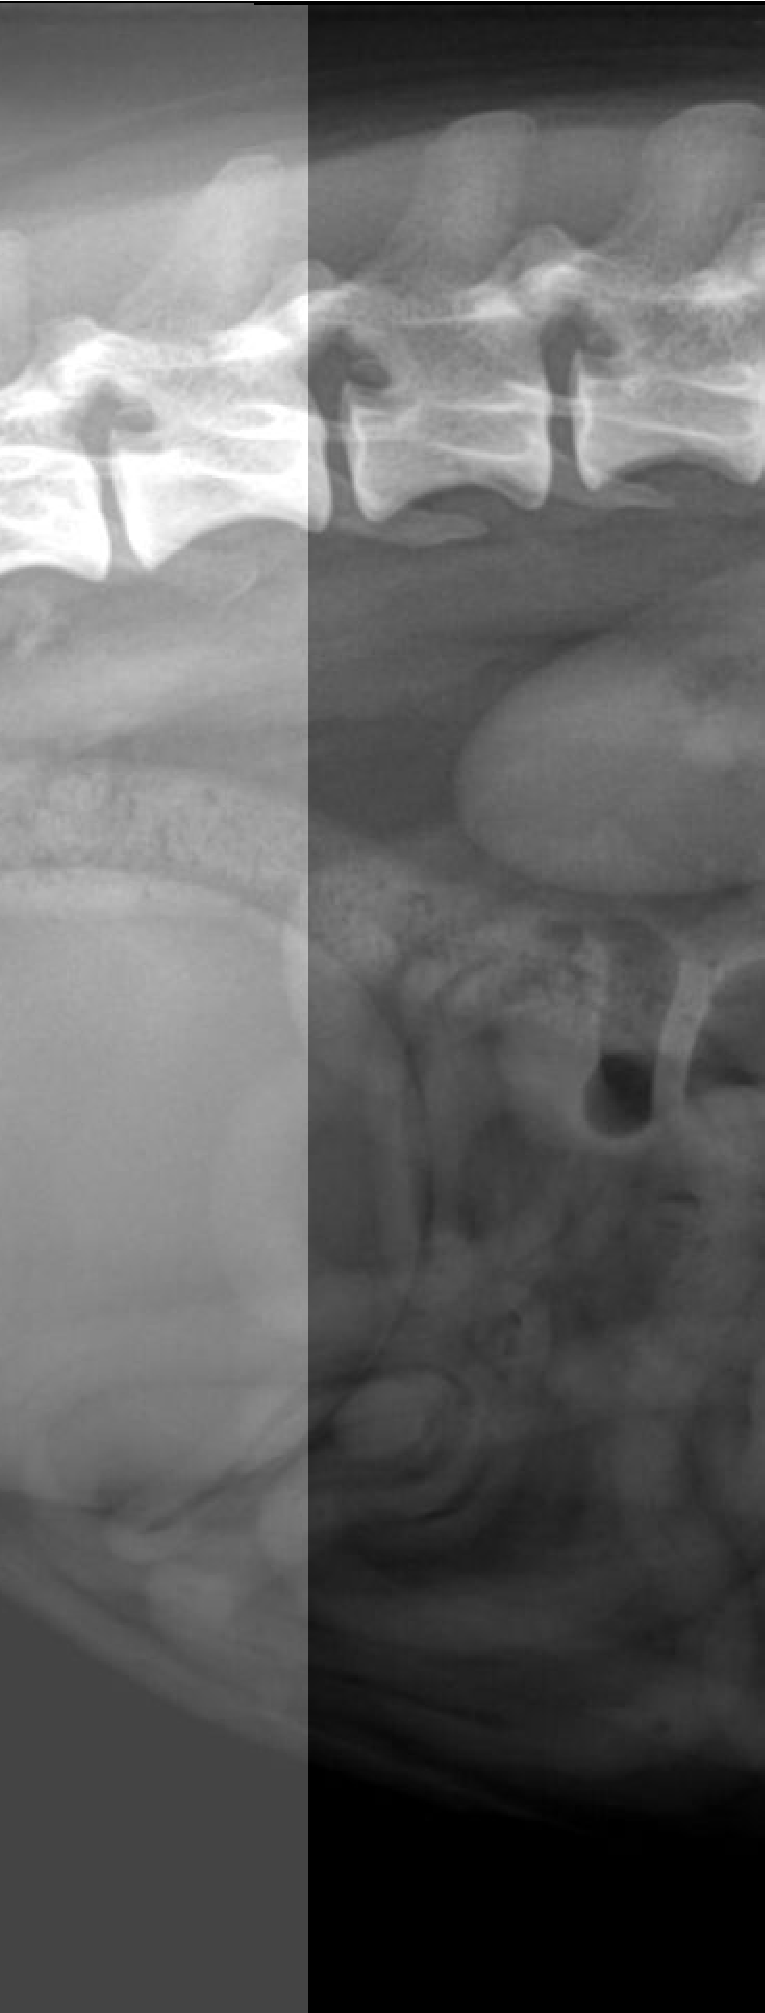
\includegraphics[scale=0.30]{2.mainmatter/2.Methodology/figures/raw-composite-image}} \quad
\subfloat[]{\label{fig:pyramid-4}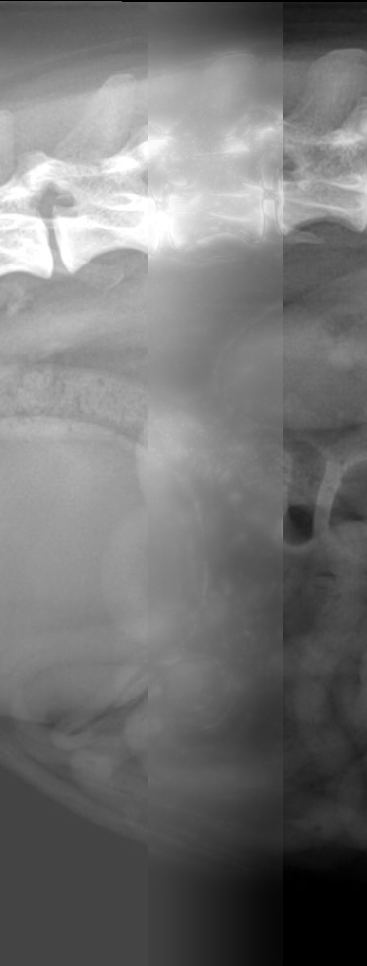
\includegraphics[scale=0.30]{2.mainmatter/2.Methodology/figures/stitched-image-pyramid-4}} \linebreak
\subfloat[]{\label{fig:pyramid-2}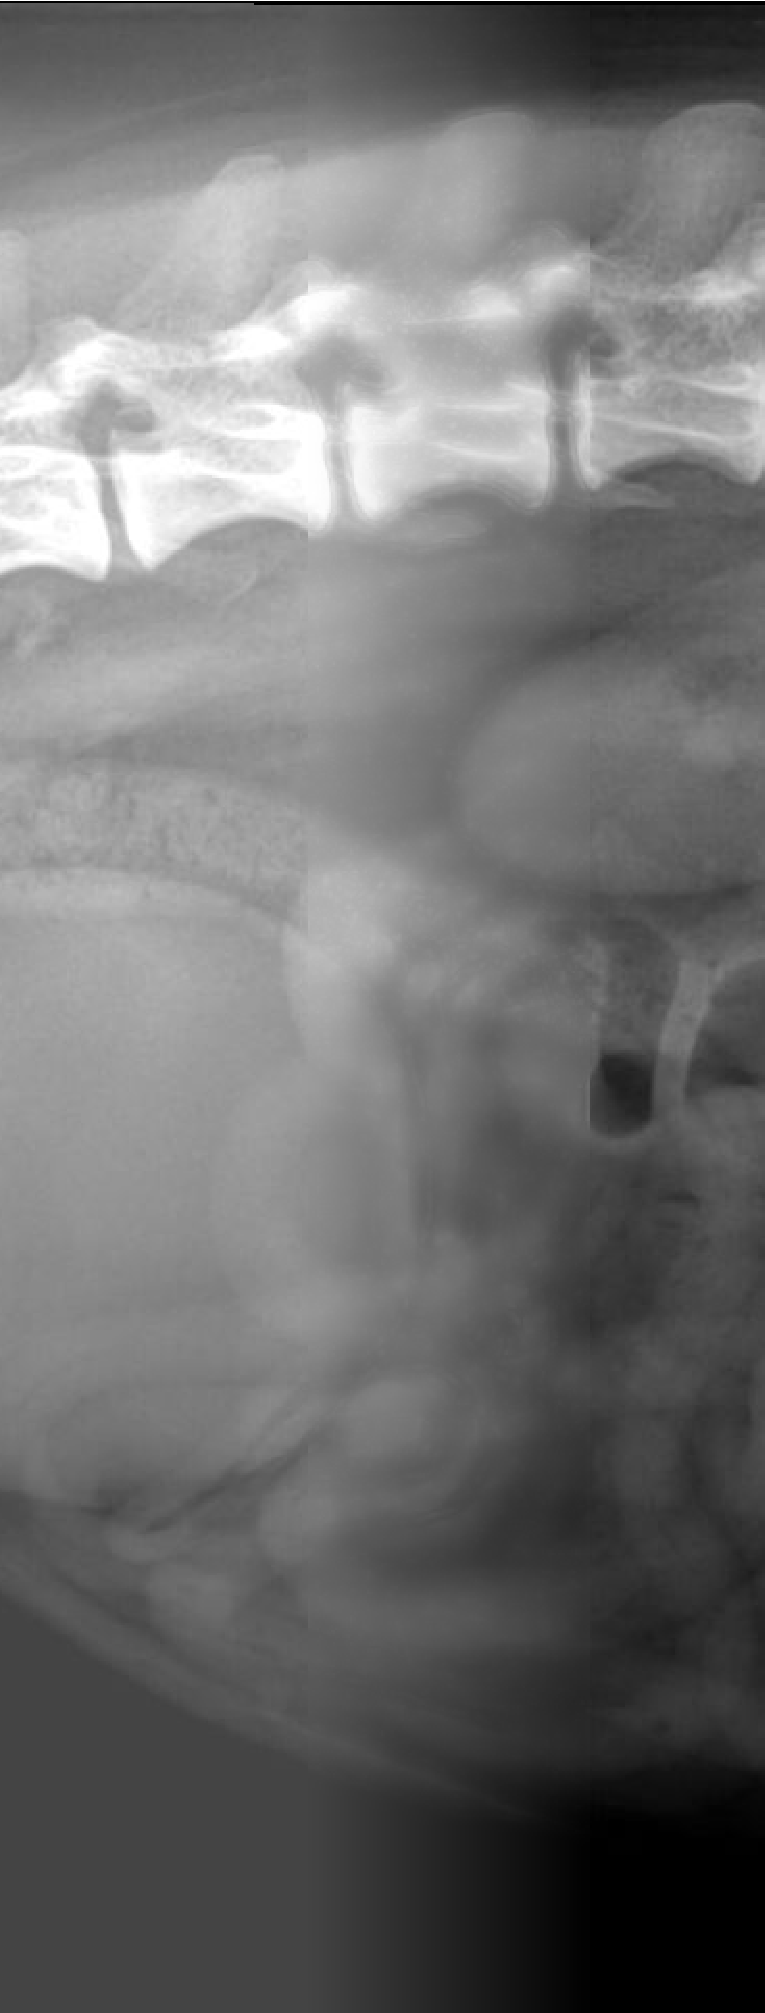
\includegraphics[scale=0.30]{2.mainmatter/2.Methodology/figures/stitched-image-pyramid-2}} \quad
\subfloat[]{\label{fig:alpha}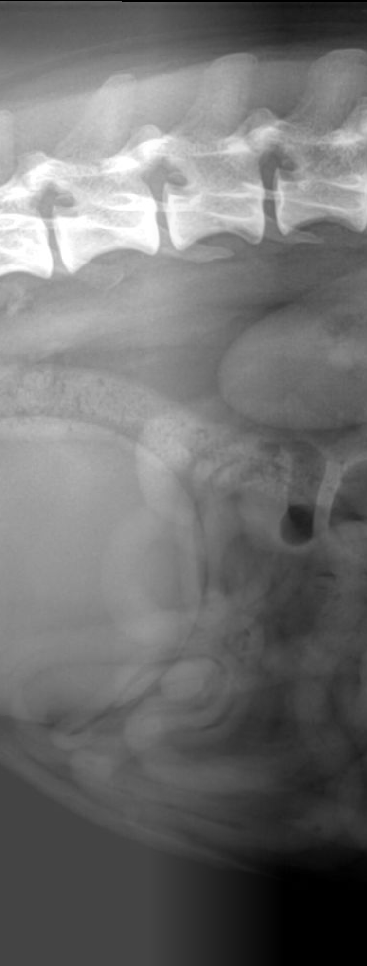
\includegraphics[scale=0.30]{2.mainmatter/2.Methodology/figures/stitched-image-alpha}}
\caption[Alpha Blending versus Pyramid Blending]{Comparison of results of Pyramid Blending and Alpha Blending. \subref{fig:raw-composite} is the composite image, \subref{fig:pyramid-4} is level 4 pyramid blended, \subref{fig:pyramid-2} is level 2 pyramid blended and \subref{fig:alpha} is alpha blended image. The blurring effect in Pyramid Blending is undesirable because it loses image information.}%
\label{fig:alpha-vs-pyramid}%
\end{figure}

\subsection{Blending Masks}
In the above section, I found alpha blending is faster and gives more accurate result as compared to pyramid blending. In this section, I will carry out experiments on the images with complex alignments. The horizontal or vertical blending for the image shown in figure~\ref{fig:multi-raw-composite-image} produces visible seams shown in figure~\ref{fig:single-alpha}.\\

\begin{figure}[H]%
\centering
\subfloat[]{\label{fig:multi-raw-composite-image} 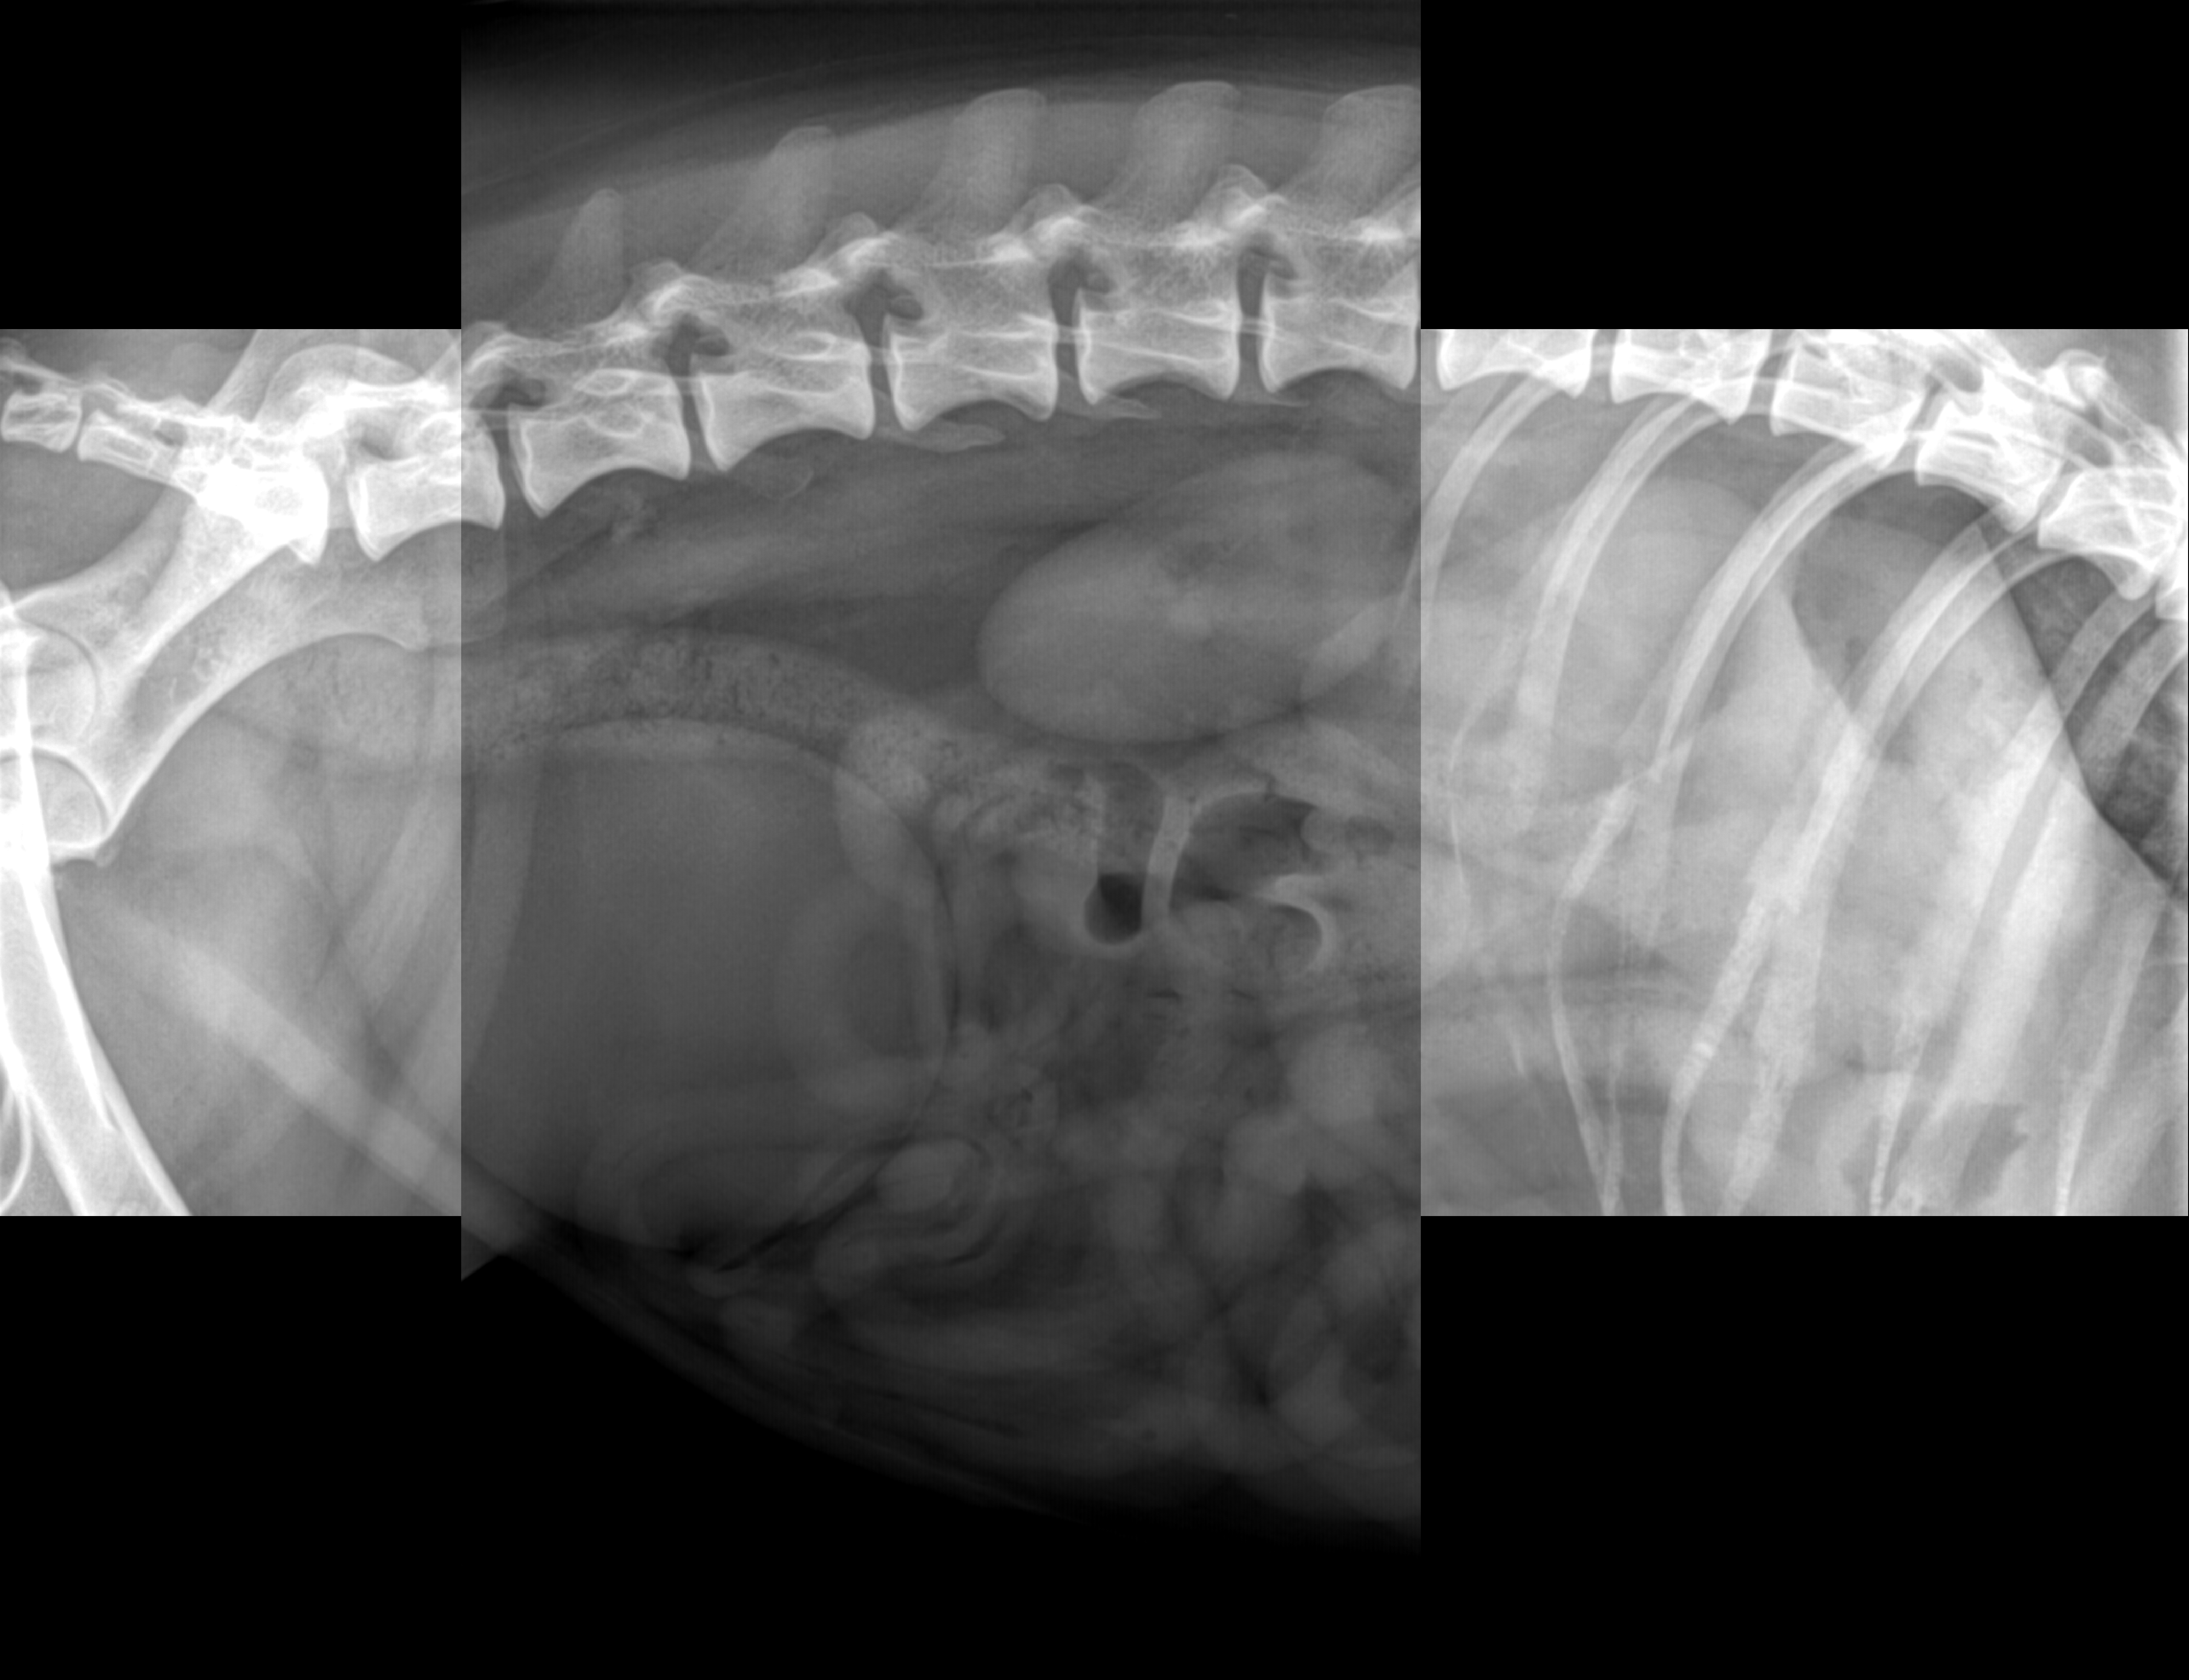
\includegraphics[scale=0.09]{2.mainmatter/2.Methodology/figures/multi-raw-composite-image}}
\subfloat[]{\label{fig:single-alpha} 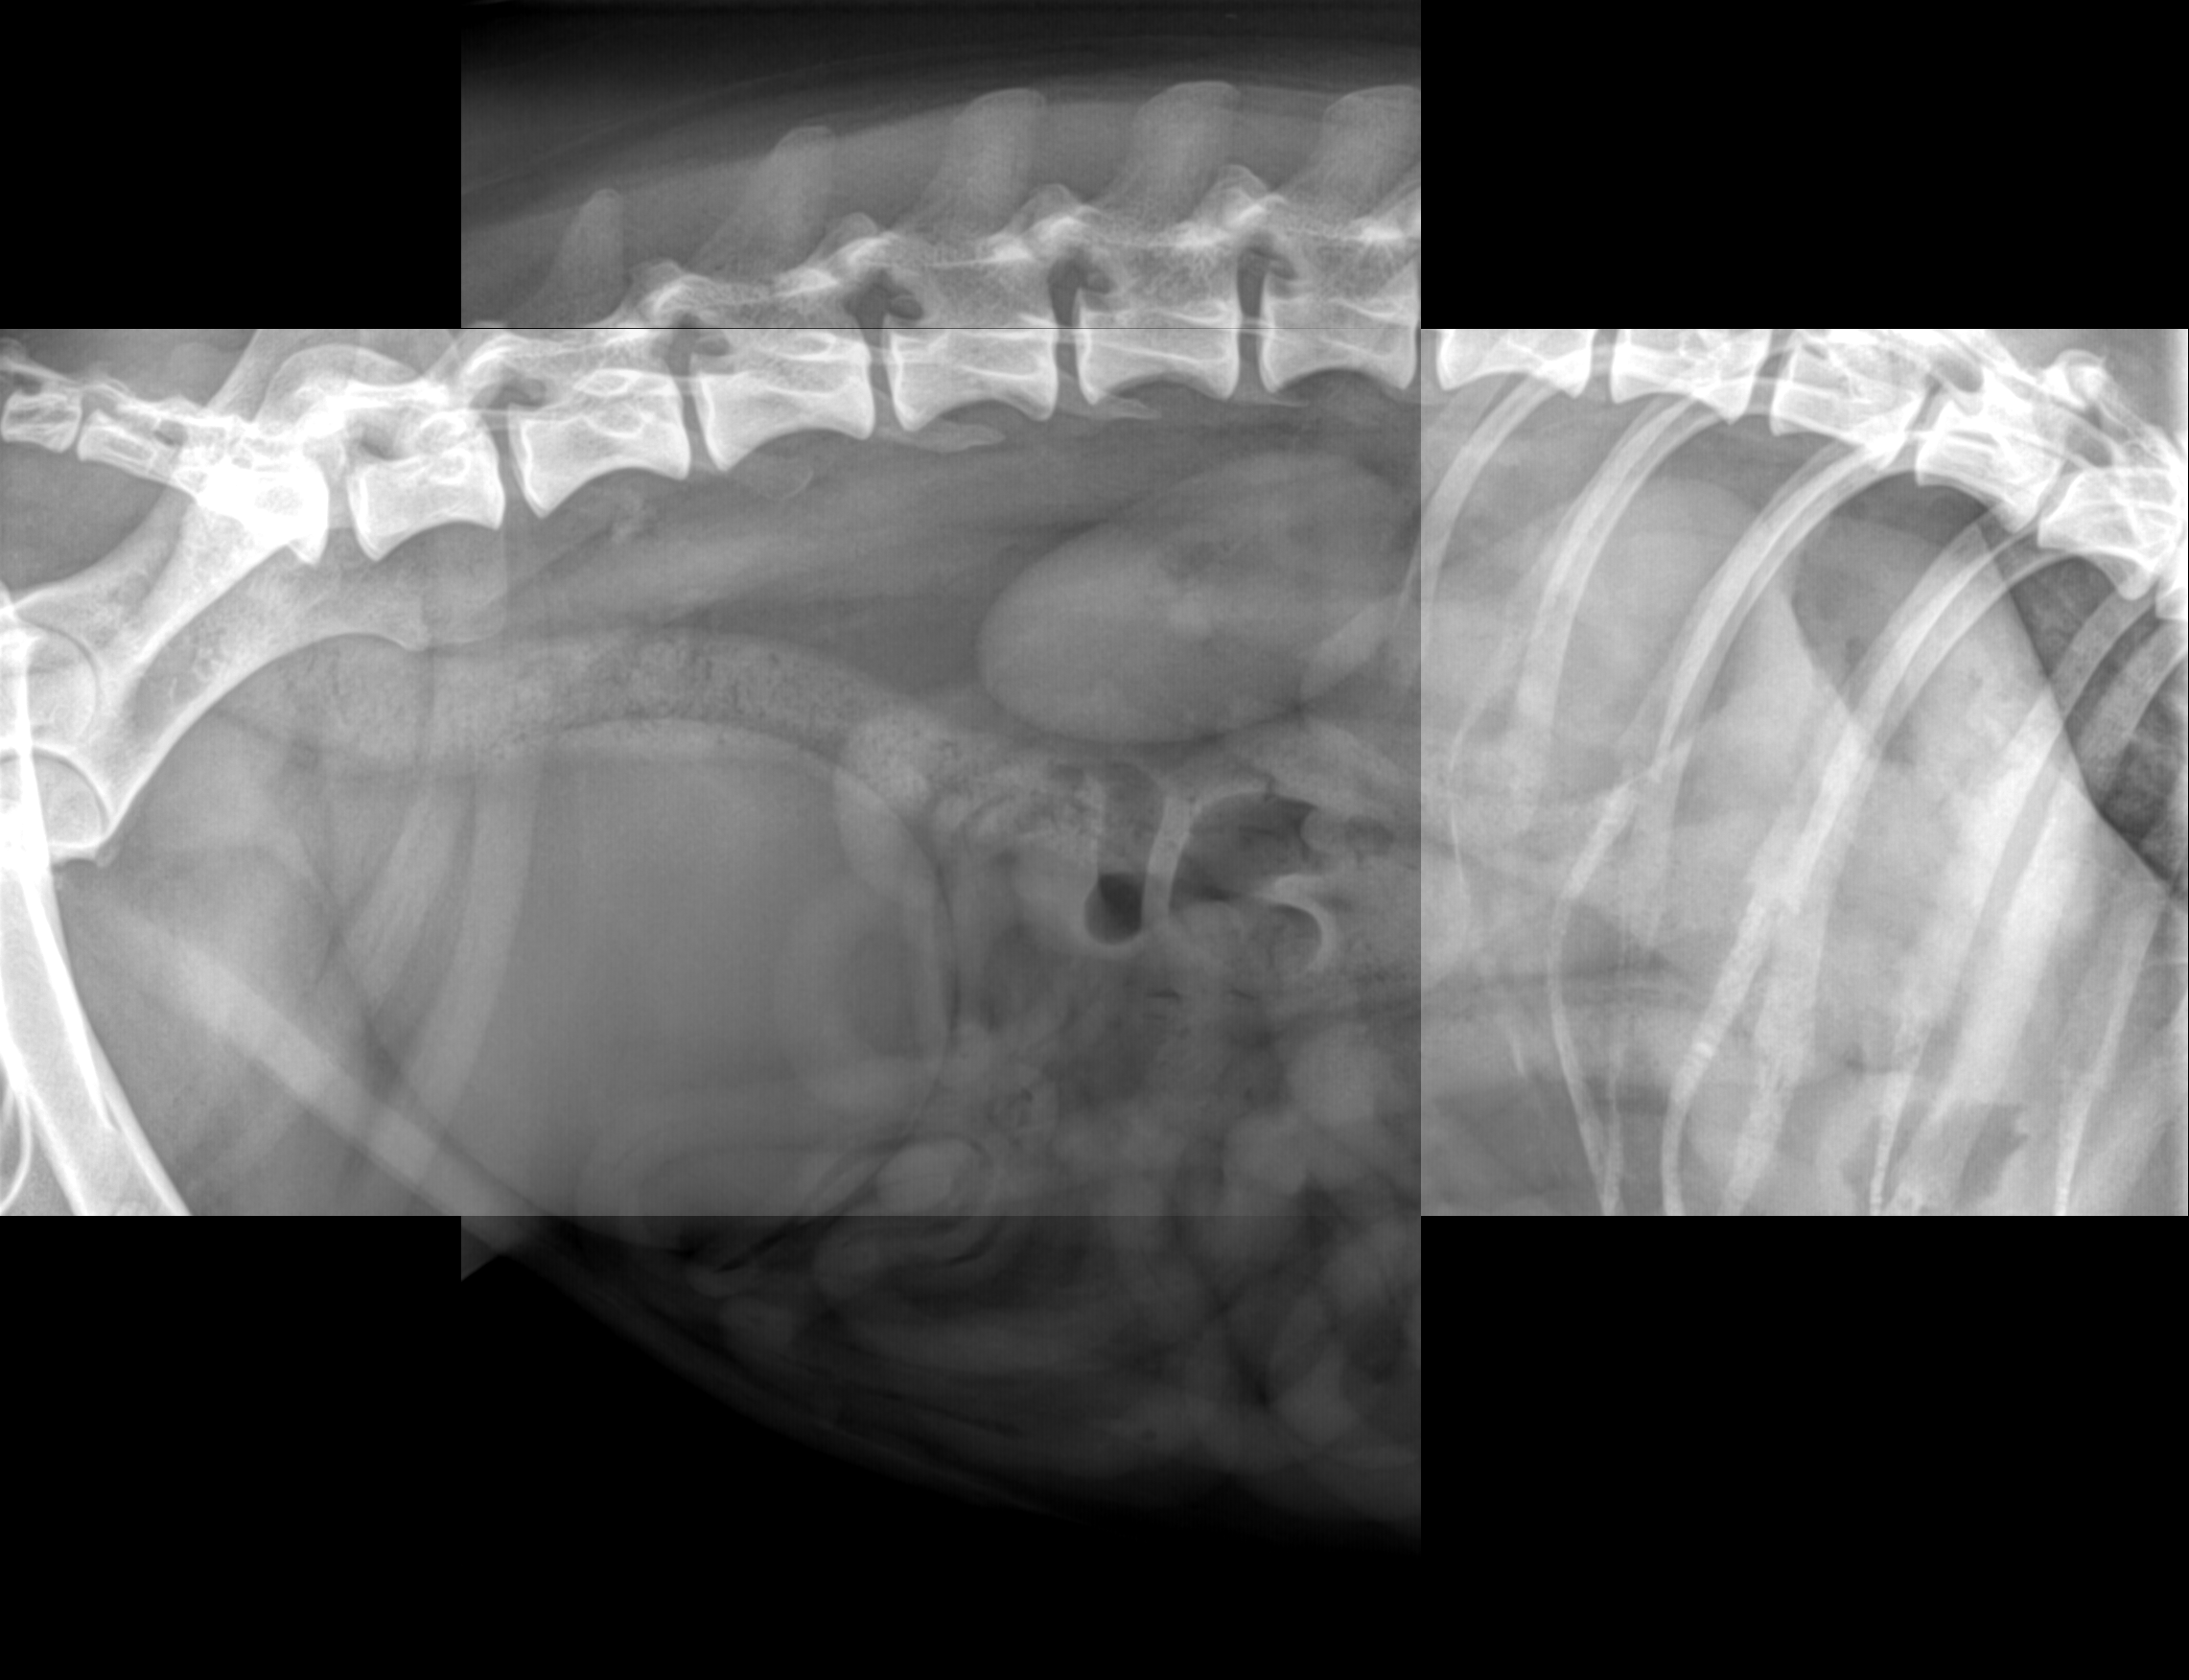
\includegraphics[scale=0.09]{2.mainmatter/2.Methodology/figures/single-alpha}}
\caption[Complex Alignment]{Figure \subref{fig:multi-raw-composite-image} is raw composite image, figure \subref{fig:single-alpha} is horizontally blended image. The seams are clearly visible on the join of the images.}%
\label{fig:blending-complex-alignment}%
\end{figure} 

\noindent So, to remedy this problem, a \emph{modified alpha blending method} has been implemented in which we create four blending masks (\emph{left}, \emph{top}, \emph{right}, \emph{bottom}) as shown in figure~\ref{fig:blending-masks}. The values in the mask indicates the effect of the image in the corresponding blending pixel (i.e. the higher value, the higher effect). For example, the left blending mask has higher values (shown white in the image) in left side means left image will have higher effect in the left side of the blended region to remove discontinuities in the composite image.\\


\begin{figure}[H]%
\centering
\subfloat[Left]{\label{fig:blending-mask1} 
\includegraphics[scale=0.1]{2.mainmatter/2.Methodology/figures/blending-mask-0}}
\subfloat[Top]{\label{fig:blending-mask2} 
\includegraphics[scale=0.1]{2.mainmatter/2.Methodology/figures/blending-mask-1}}
\subfloat[Right]{\label{fig:blending-mask3} 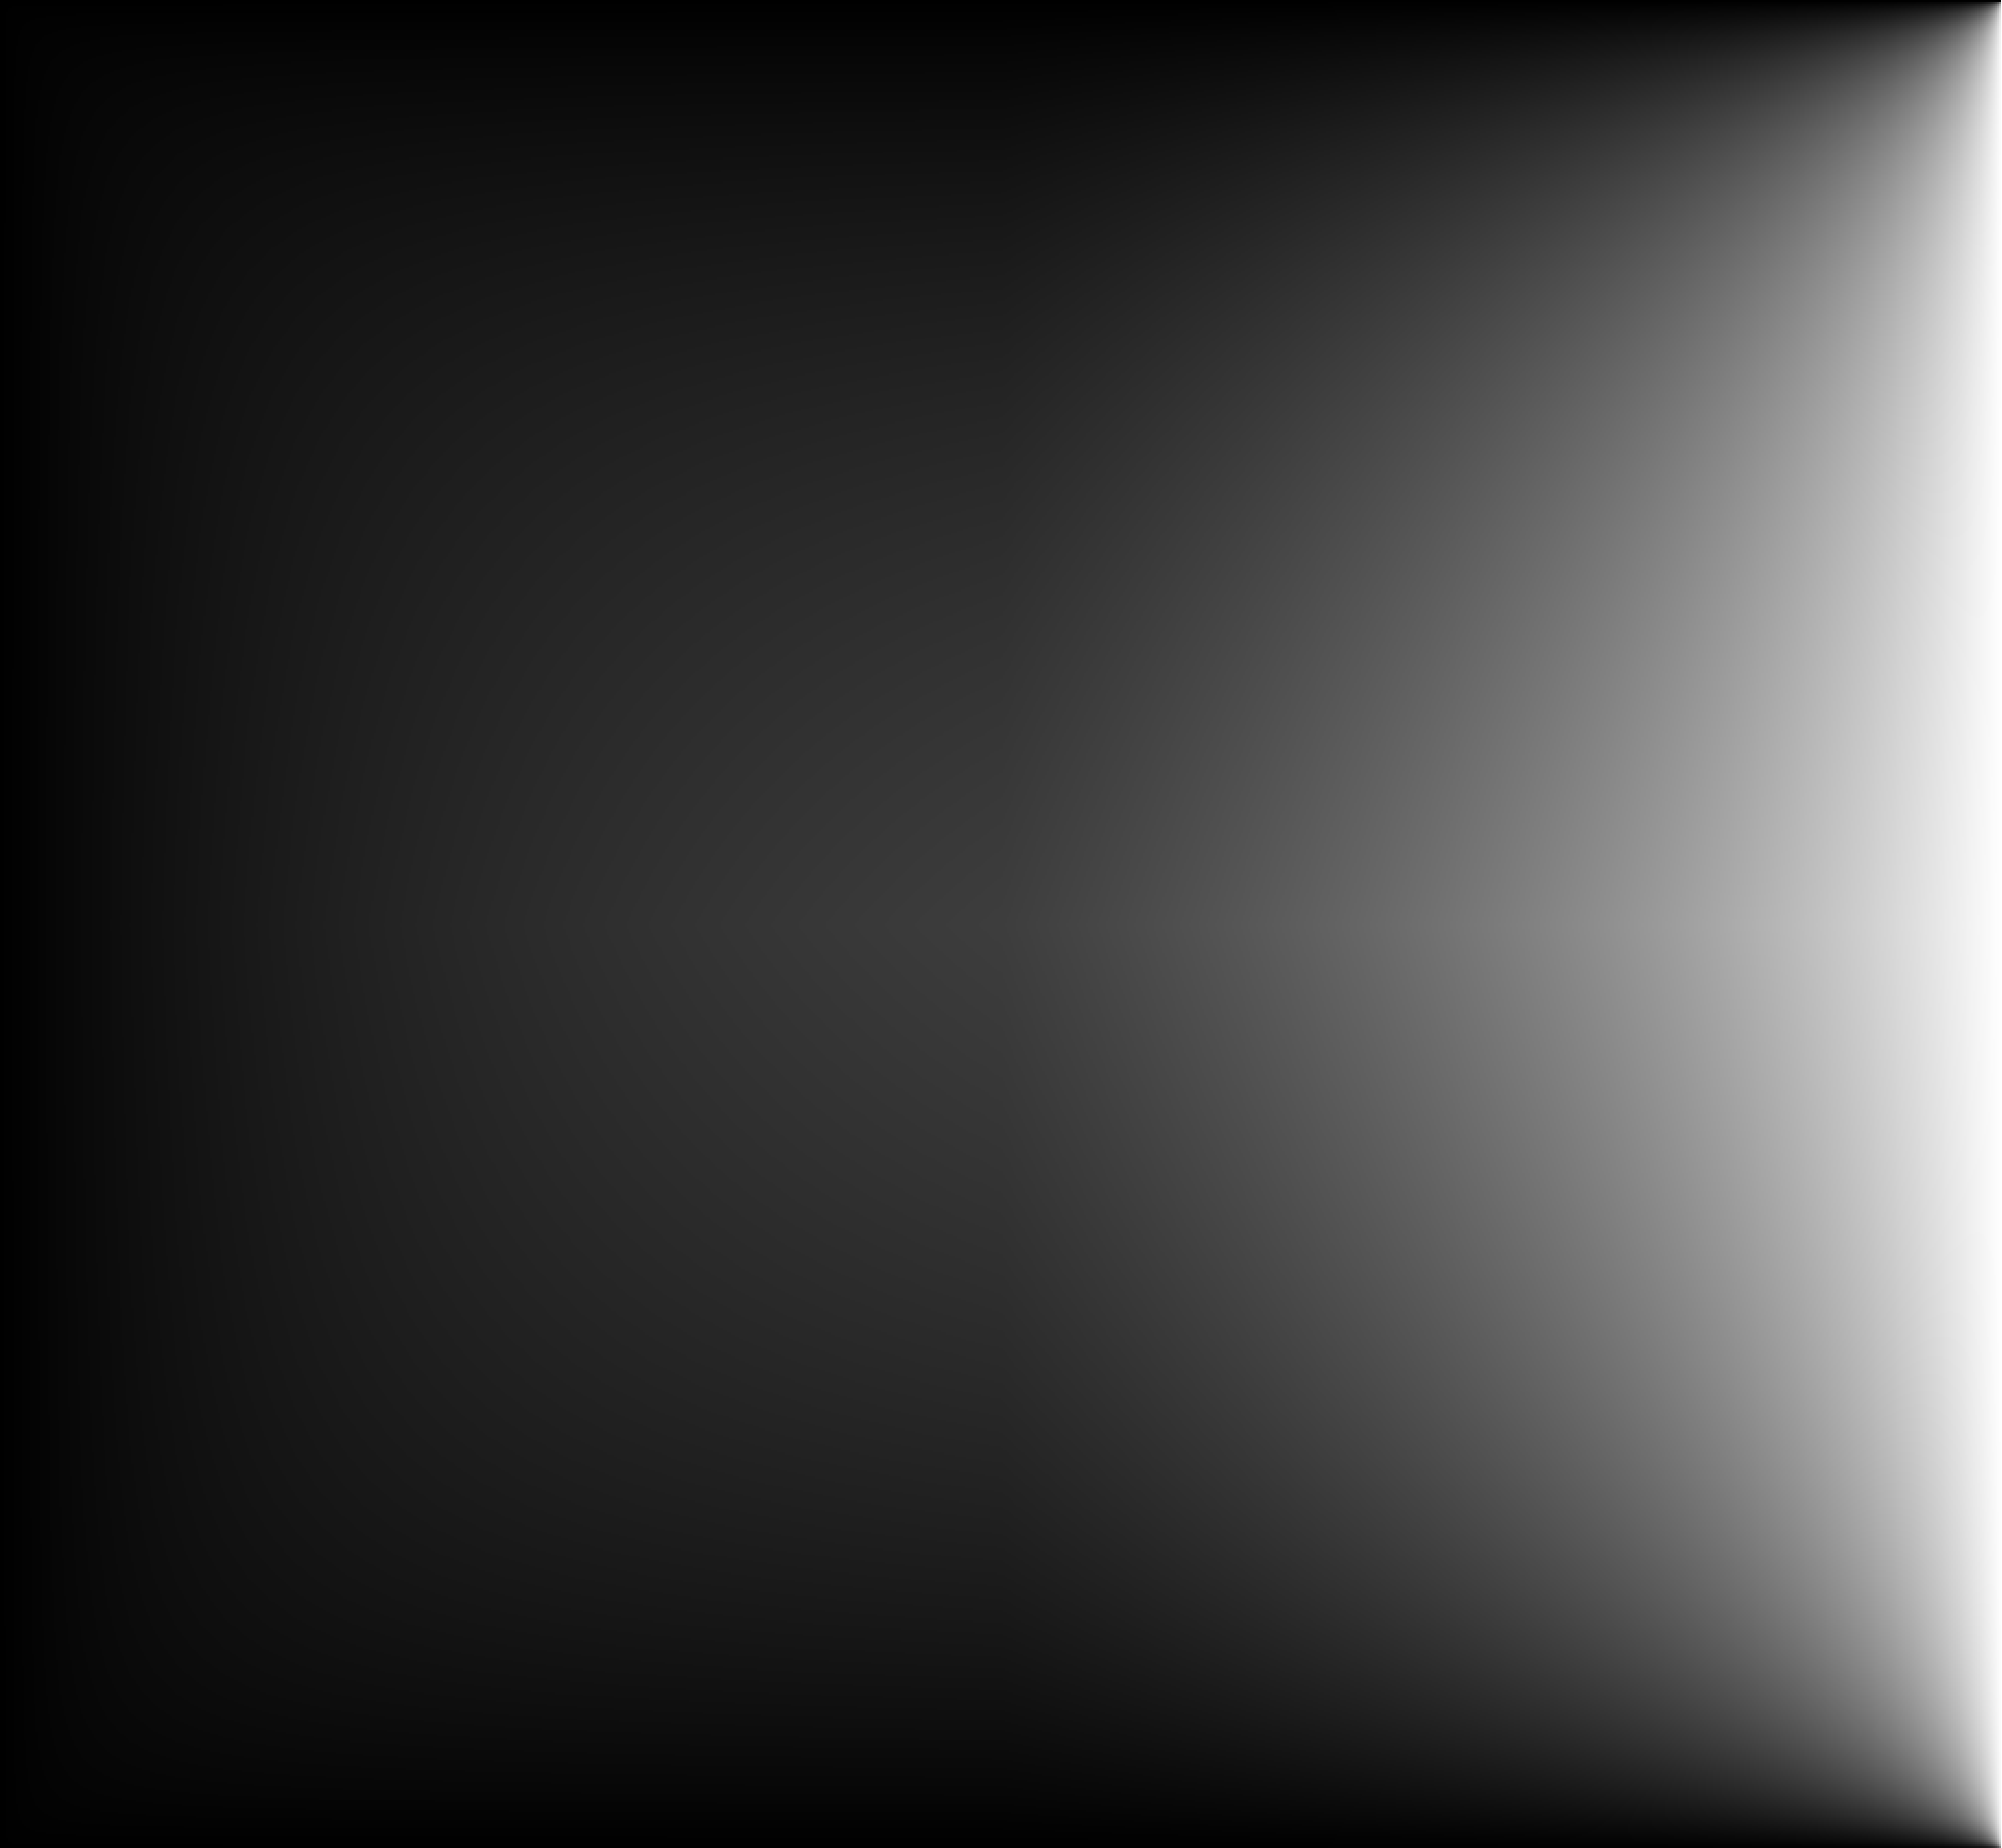
\includegraphics[scale=0.1]{2.mainmatter/2.Methodology/figures/blending-mask-2}}
\subfloat[Bottom]{\label{fig:blending-mask4} 
\includegraphics[scale=0.1]{2.mainmatter/2.Methodology/figures/blending-mask-3}}
\caption[Blending Masks]{Blending masks. \subref{fig:blending-mask1} is mask for left image,\subref{fig:blending-mask2},\subref{fig:blending-mask3}, \subref{fig:blending-mask4} are masks for top, right and bottom images respectively.}
\label{fig:blending-masks}
\end{figure} 

\noindent The blended image using multiple blending masks is shown in figure~\ref{fig:blending-complex-alignment} which is far better than the image produced with either horizontal or vertical blending (compare images:~\ref{fig:single-alpha} and~\ref{fig:blending-complex-alignment})

\begin{figure}[H]%
\centering
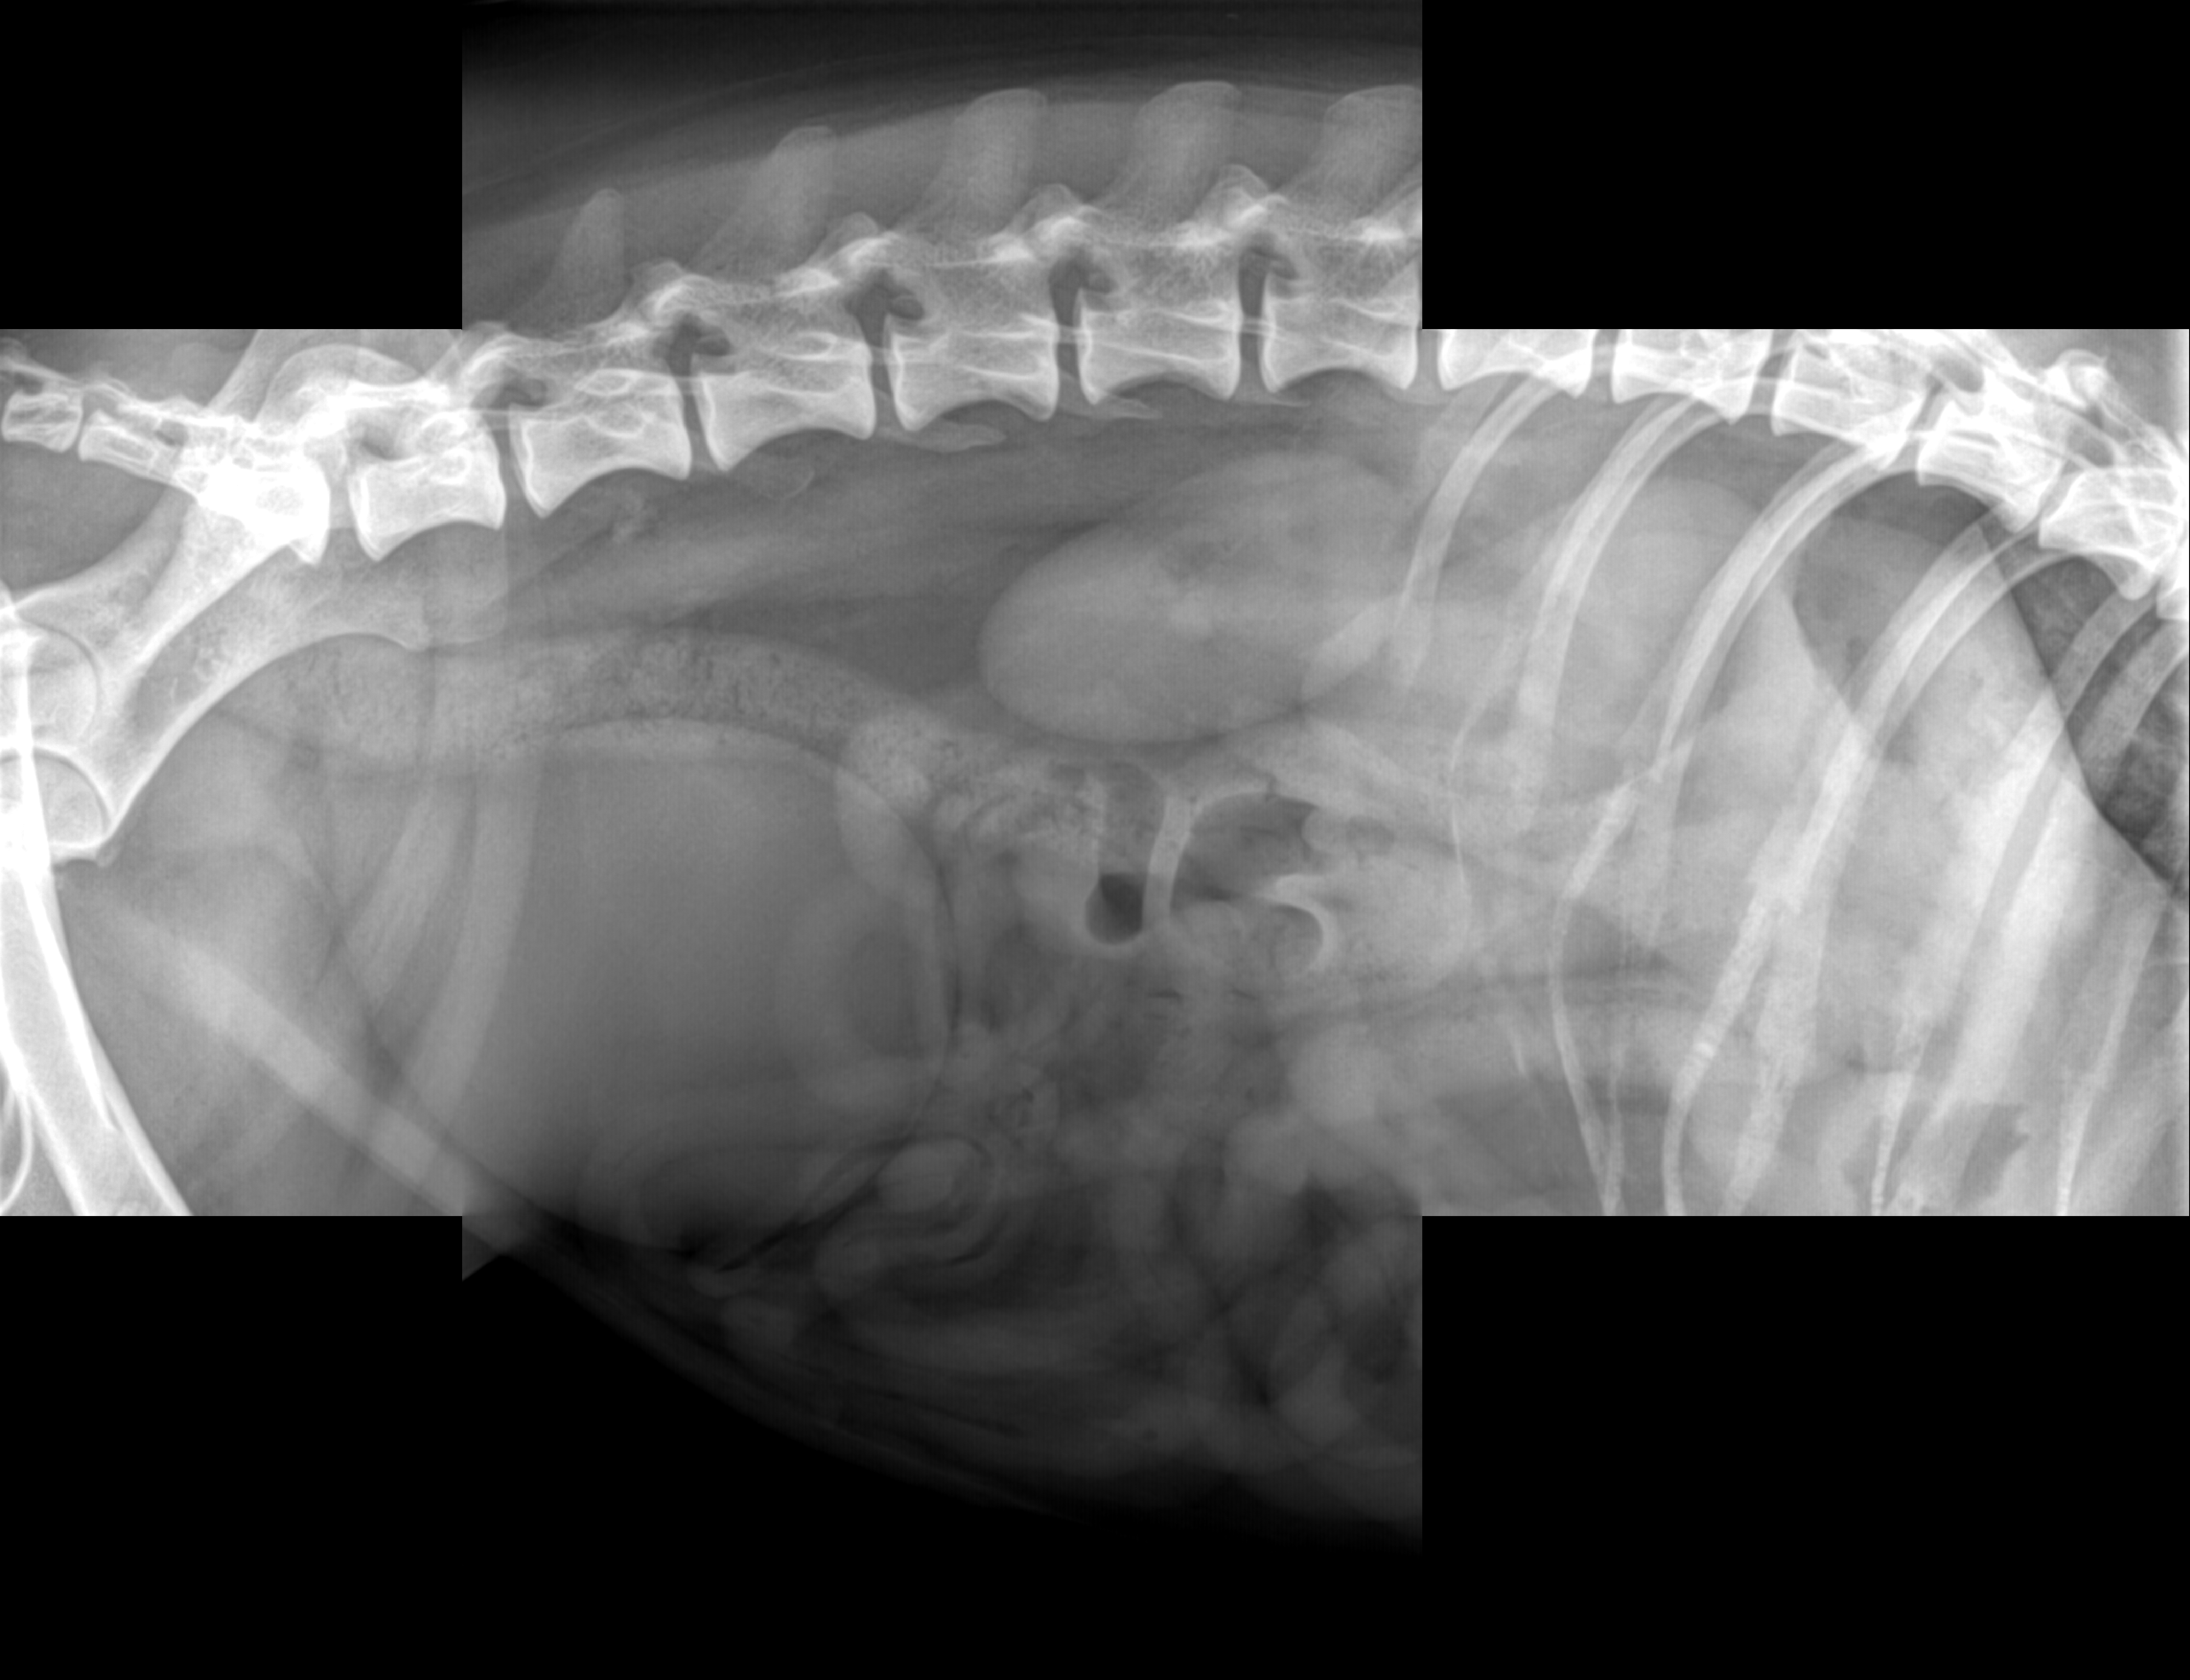
\includegraphics[scale=0.15]{2.mainmatter/2.Methodology/figures/multi-alpha}
\caption[Blending with Masks]{Use of multiple blending masks gives better blending result.}%
\label{fig:blending-complex-alignment}%
\end{figure}




